Para determinar la carga especifica del electron, se pone a un electron que se mueve a una velocidad $v$ bajo el campo magnetico 
generado por un par de Bobinas de Helmholtz, dichas bobinas representan una de las configuraciones más
simples para generar un campo magnético relativamente constante. Estas bobinas consisten en dos bobinas circulares coaxiales de igual
radio, el cual es igual a la distancia entre los planos de las bobinas.



\begin{figure}[H]
    \centering
    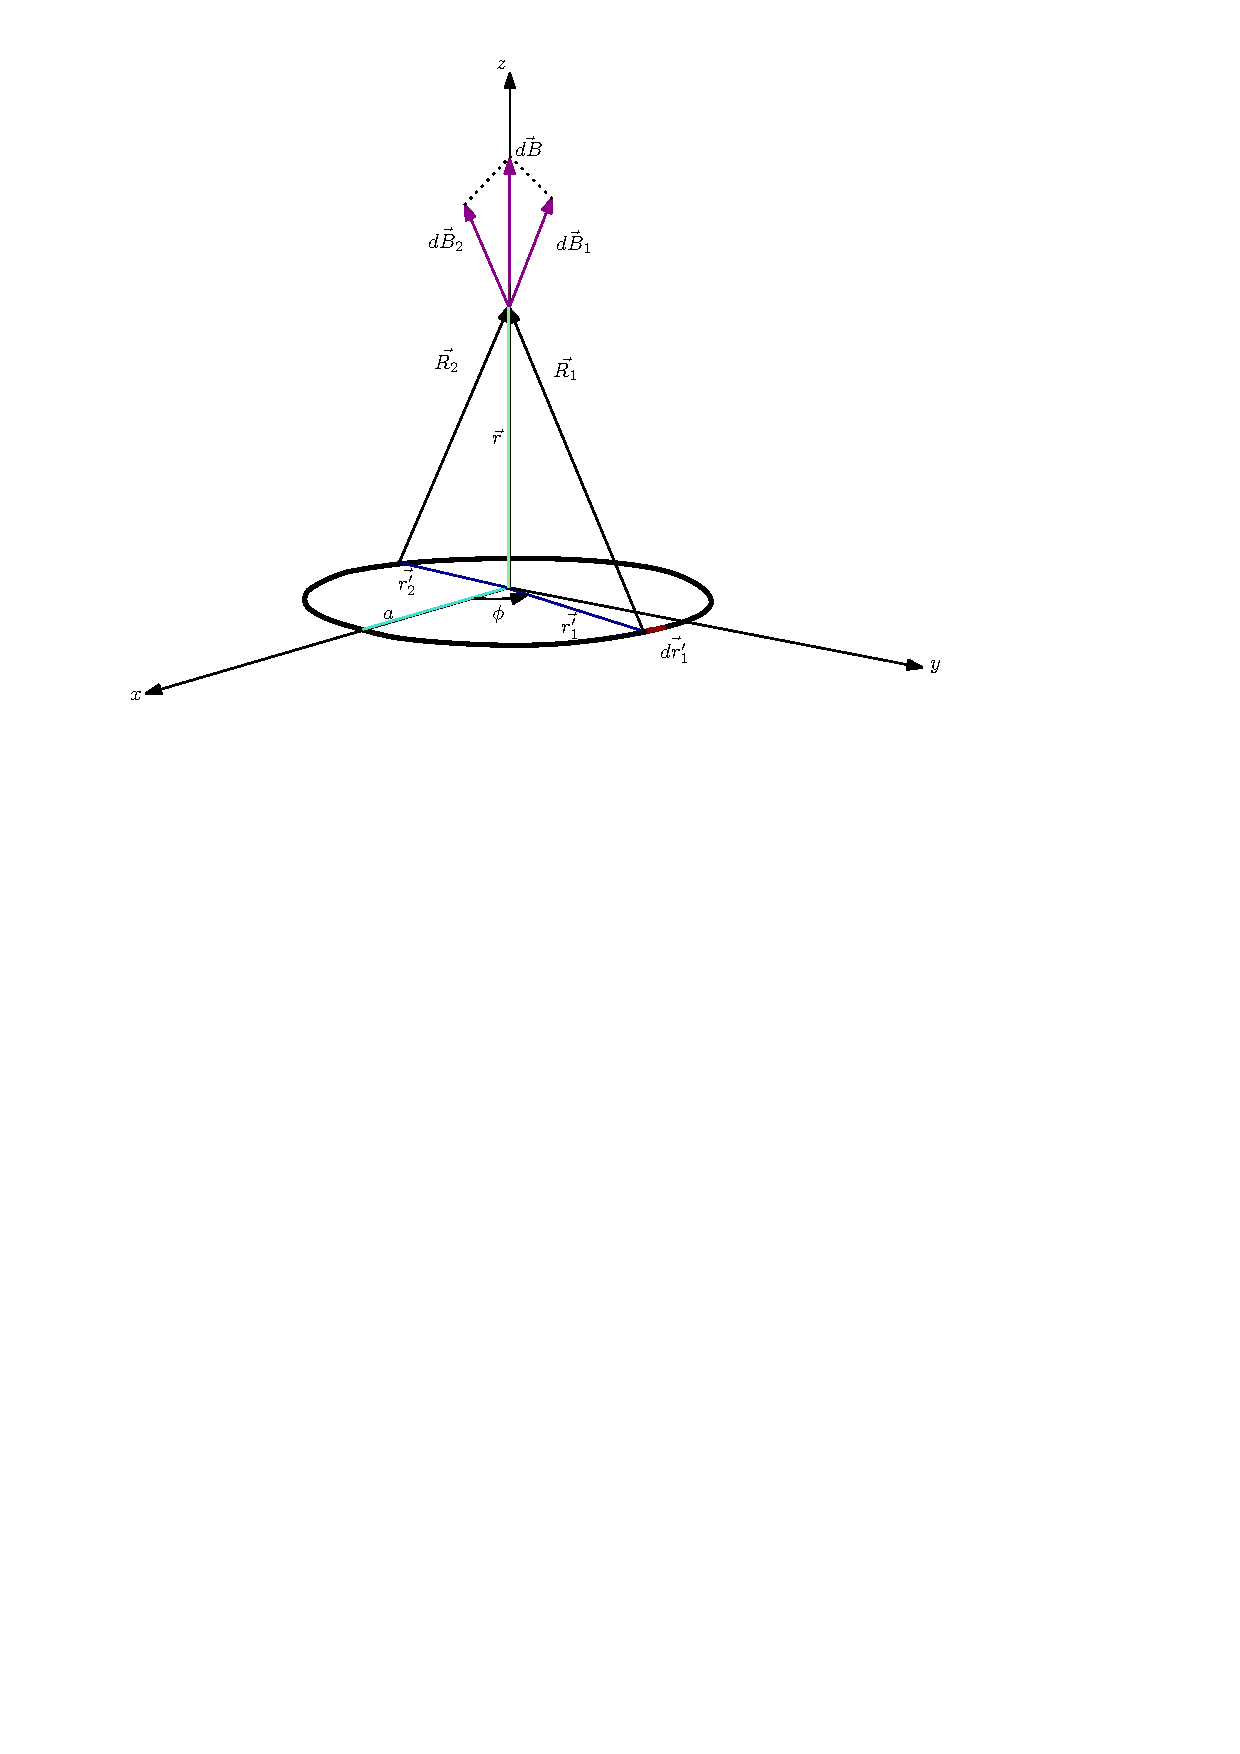
\includegraphics[width=0.8\linewidth]{images/Campo de una espira.pdf}
    \caption{Campo magnético de una espira.}
    \label{fig:una_espira}
\end{figure}

Para calcular el campo magnético generado por estas bobinas, primero se determina el campo producido por una de ellas. En este caso, se considera una espira por la que circula una corriente eléctrica constante $I$ en el tiempo. Partimos de la expresión diferencial de la ley de Biot-Savart:

\begin{equation}\label{eq:Biot-Savart}
    d\mathbf{B}(\mathbf{r}) = \frac{\mu_0 I}{4 \pi} \frac{d\mathbf{l} \times \mathbf{R}}{R^{3}}
\end{equation}

Donde:

$d\mathbf{l}=a d\phi \hat{\phi}$ 

$\mathbf{R}=\mathbf{r}-\mathbf{r'}$ 

$\mathbf{r}=z\hat{e_{z}}-a\hat{e_{\rho}}$

$R=\sqrt{z^{2}+a^{2}}$ 

Por lo que reemplazando se tiene que:

\begin{equation} 
    d\mathbf{B}(\mathbf{r}) = \frac{\mu_{0}I}{4\pi} \frac{(a d\phi z \hat{\rho}) + (a^{2}d\phi \hat{z})}{(z^{2}+a^{2})^{3/2}}
\end{equation} 

Al integrar se obtiene el valor de $\mathbf{B}(\mathbf{r})$ y por la simetría del problema se evidencia que $\mathbf{B}(\mathbf{r}) = B(r)\hat{z}$, por lo que se obtiene:

\begin{equation} 
	\mathbf{B}(\mathbf{r}) = \frac{\mu_{0}I}{4 \pi} \frac{a^{2}}{(z^{2}+a^{2})^{3/2}} \hat{e_{z}} \int _{0}^{2 \pi} d\phi
\end{equation}

Lo que da como resultado:

\begin{equation} 
    \mathbf{B}(\mathbf{r}) = \frac{\mu_{0}I}{2} \frac{a^{2}}{(z^{2}+a^{2})^{3/2}} \hat{e}_{z}
    \label{eq:Campo_magnetico_espira}
\end{equation} 

\begin{figure}[H]
    \centering
    \begin{subfigure}[a]{0.45\textwidth}
        \centering
        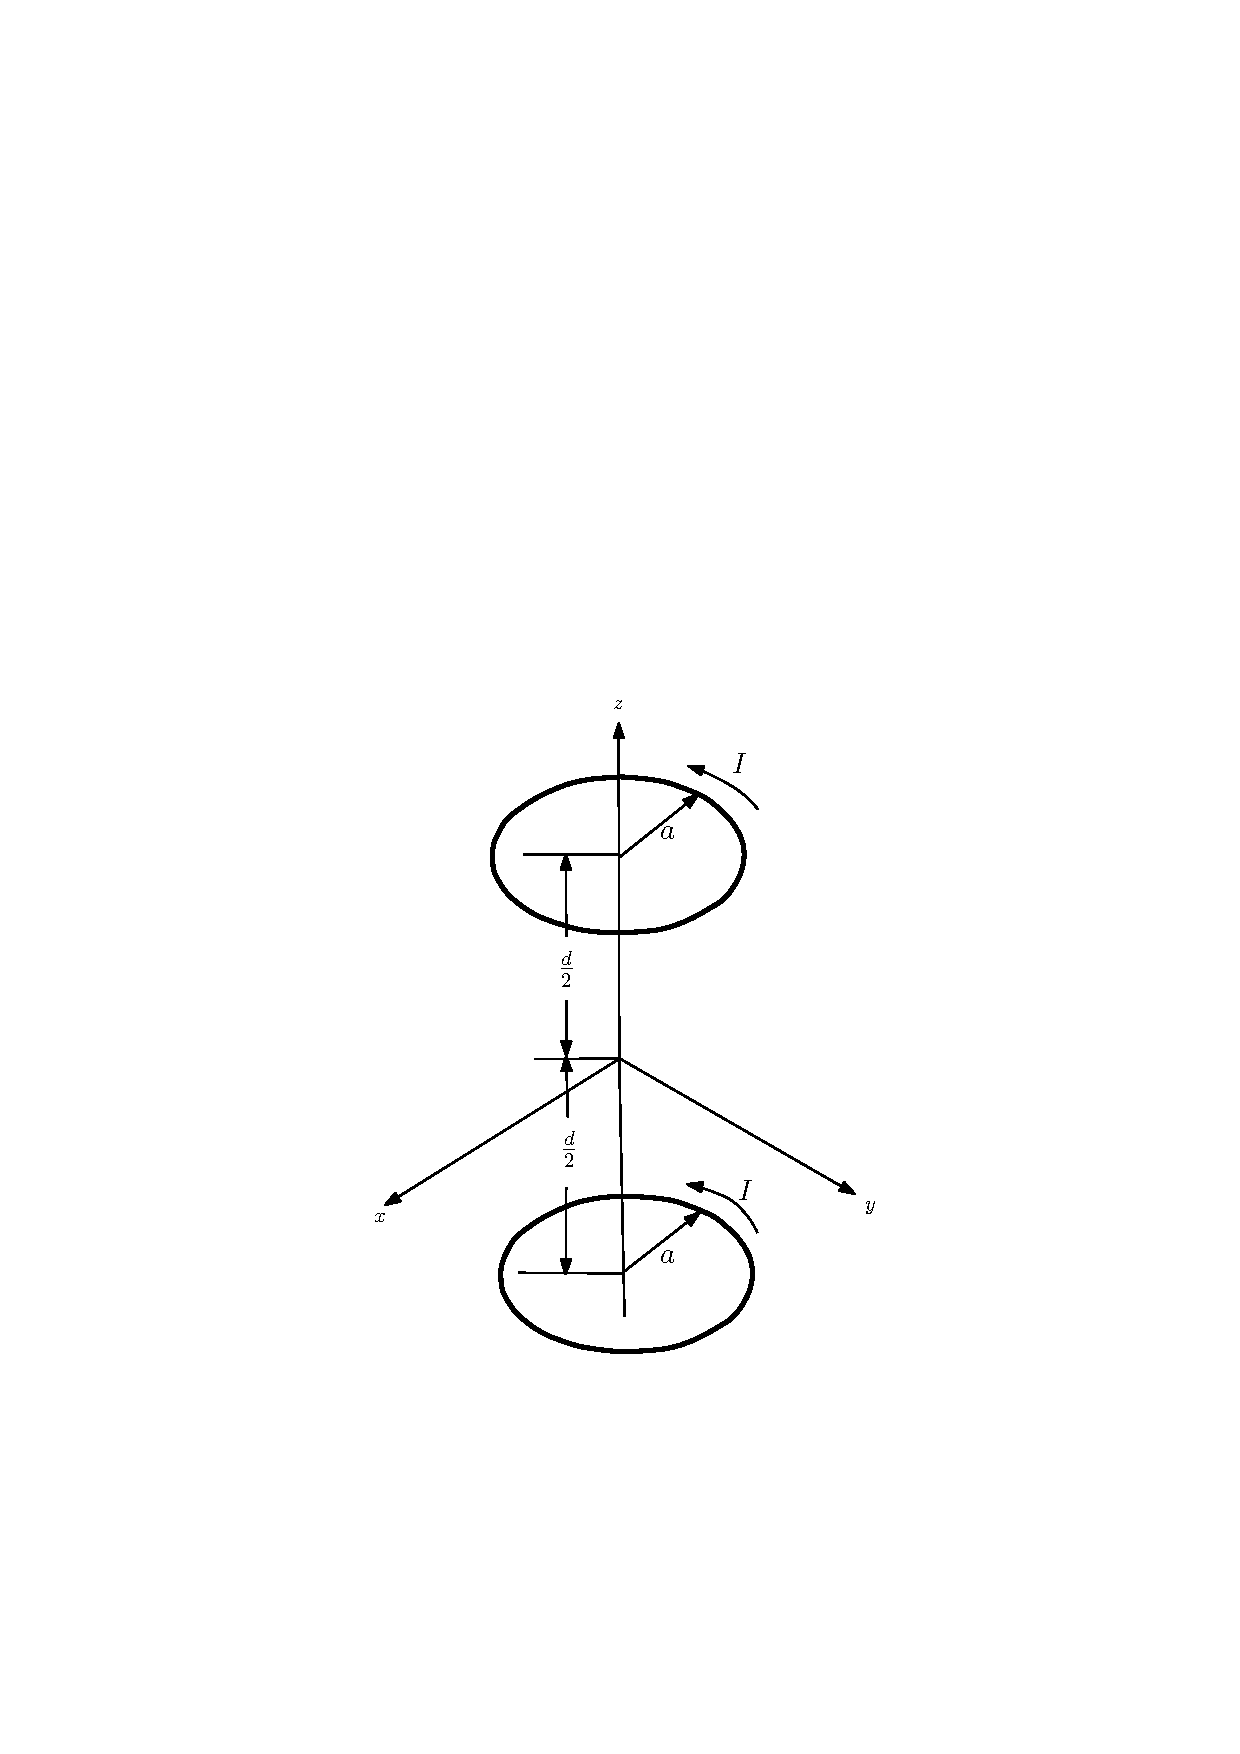
\includegraphics[width=0.6\textwidth]{images/dos espiras.pdf}
        \caption{Corriente en dos espiras}
        \label{fig:I_en_dos_espiras}
    \end{subfigure}
    \hfill
    \begin{subfigure}[b]{0.45\textwidth}
        \centering
        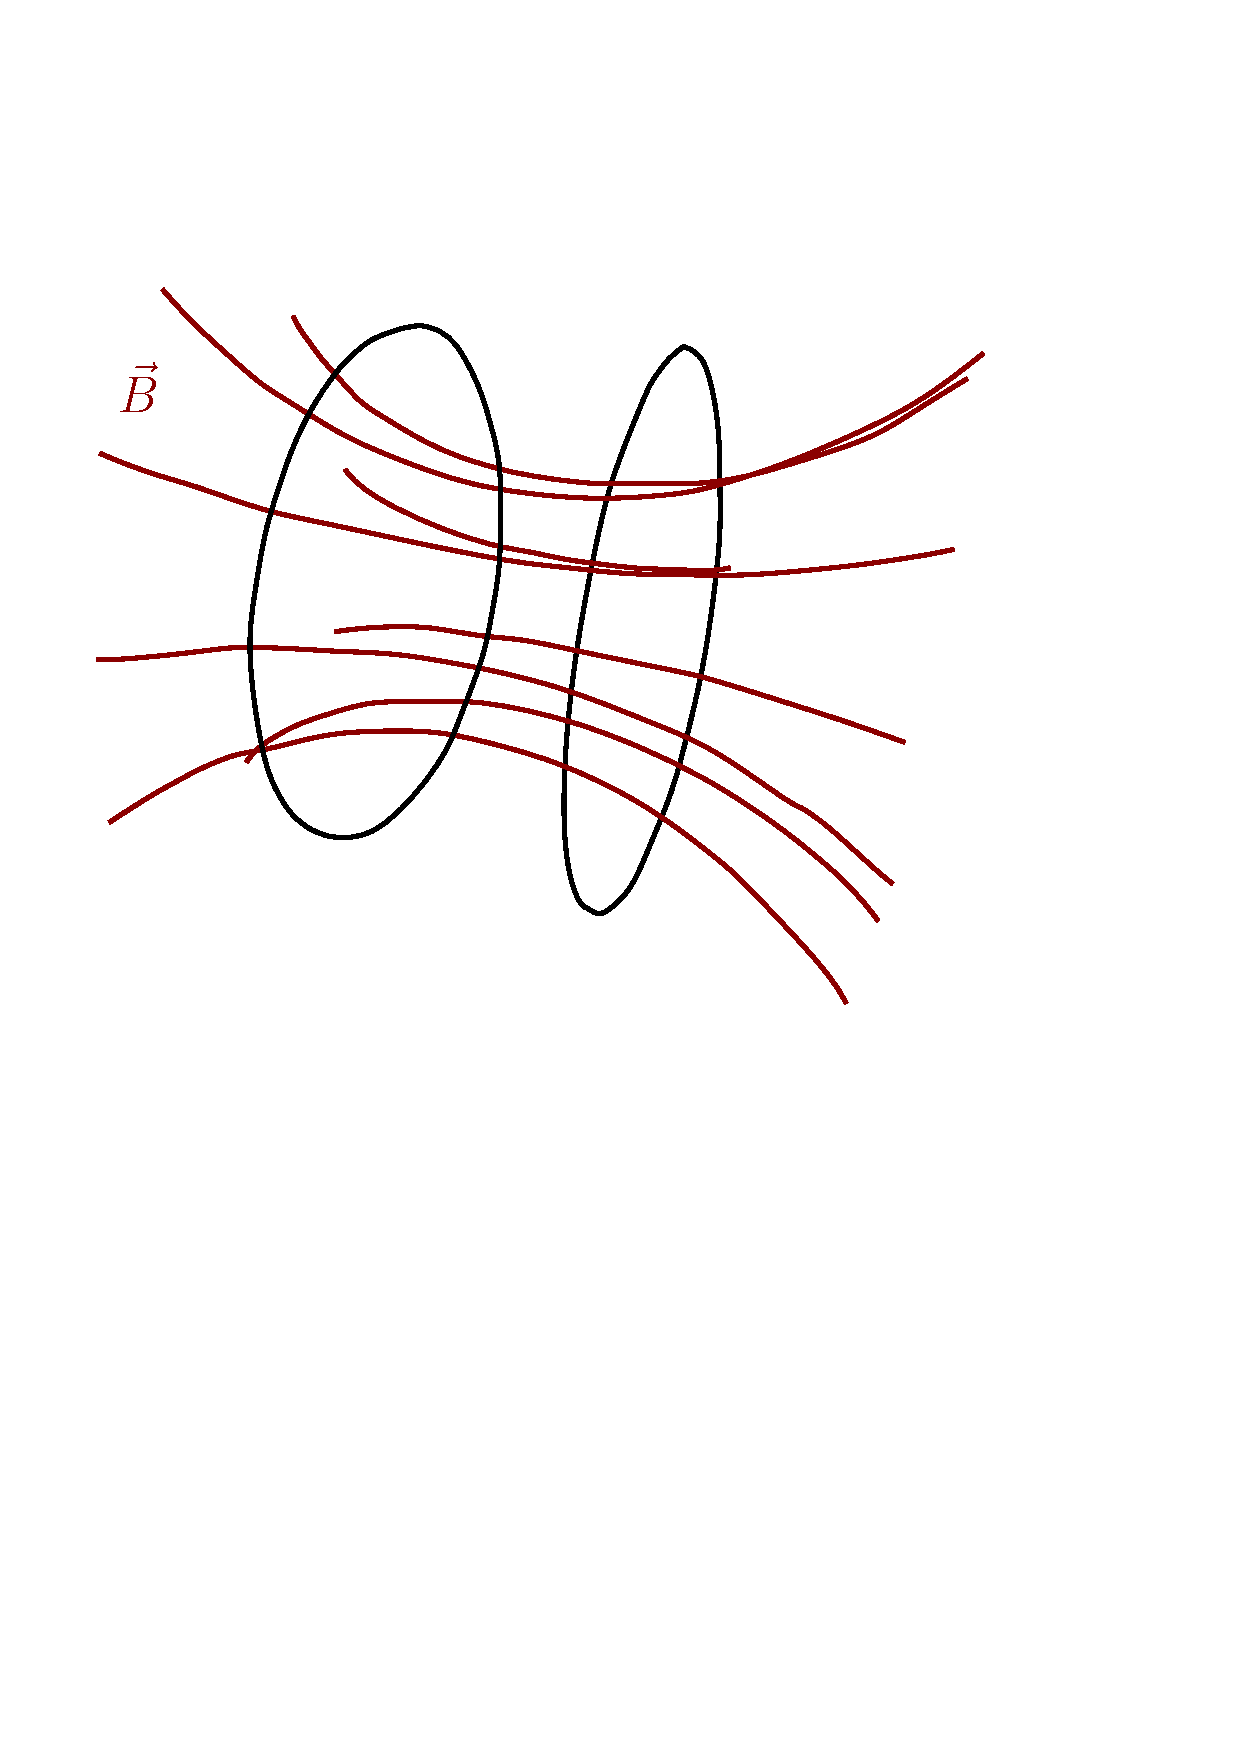
\includegraphics[width=0.6\textwidth]{images/Campo de bobinas.pdf}
        \caption{Campo magnético entre dos espiras circulares}
        \label{fig:CM_dos_espiras}
    \end{subfigure}
    \caption{Dos espiras circulares}
    \label{fig:dos_espiras}
\end{figure}

El campo magnético $\mathbf{B}$ producido por dos espiras, como se observa en la \cref{fig:dos_espiras}, donde circula una corriente estática $I$ en cada una de las espiras, se calcula sumando dos componentes del vector $\mathbf{B}$ de acuerdo al resultado de la \cref{eq:Campo_magnetico_espira}. Como resultado, se obtendrán dos términos iguales, considerando que las espiras se encuentran localizadas en $z = -d/2$ y $z = +d/2$.

\begin{equation}
\begin{aligned}
    \mathbf{B}_{z}(\rho=0,z) &= \frac{\mu_{0} I a^{2}}{2} \left[ \frac{1}{\left((z-\frac{d}{2})^{2} + a^{2}\right)^{3/2}} \right.\\
    &\quad \left.+ \frac{1}{\left((z+\frac{d}{2})^{2} + a^{2}\right)^{3/2}} \right] \hat{e}_{z}
    \label{Campo_magnetico_2espiras}
\end{aligned}
\end{equation}

Para el caso del montaje experimental, la bobinas tienen una separación igual a su radio, por lo que $d=a$. Ademas, el has de electrones 
se hubica en el centro de las bobinas, es decir, z=0. Teniendo en cuenta todas esta consideraciones, se llega a que el campo magnetico producido por las bobinas en el haz de electrones es: 

\begin{equation}
    \mathbf{B}_{z}(\rho=0,z=0)= \frac{8 n \mu_{0} I}{5 \sqrt{5} R}
    \label{Campo_magnetico_enHaz}
\end{equation}

Donde R=a.



